\chapter{The QRSim Plume Modelling Scenarios}
The general plume modeling scenario as tackeled in this thesis is part of the 
QRSim quadrotors simulator \parencite{denardi2013rn}. Several task variations 
were proposed from which I chose a selection and to which I added some 
modifications of my own.  The task scenarios can be classified along four 
dimensions: type of dispersion (G, D), presence of sensor noise (NF, SN), single 
or multiple pollutant sources (SS, MS), single or multiple vehicles (SV, MV).

As long as not otherwise noted location vectors are in the NED (north, east, 
down) reference frame.  Hence, the height of a location $\vc x = (x_1, x_2, 
x_3)\Tr$ is given by $-x_3$.

The most simple scenario is a Gaussian (G) plume without wind as shown in 
Figure~\ref{fig:SS-G}.  The pollutant is emitted at a constant rate resulting in 
a three-dimensional (potentially non-isotropic) Gaussian plume distribution.  
Given a source location $\vc s$, covariance matrix $\mat \varSigma$, and 
emission rate $Q$ in \si{\gram\per\second} the concentration $c(\vc x)$ at 
location $\vc x$ is given as
\begin{equation}
    c(\vc x) = Q \cdot \si{\second\per\meter^3} \cdot \exp\!\del{-\frac{1}{2} 
        (\vc x - \vc s)\Tr \mat \varSigma^{-1} (\vc x - \vc s)}.
\end{equation}

\begin{figure}
    \centering
    \subfigure[Single source 
    Gaussian]{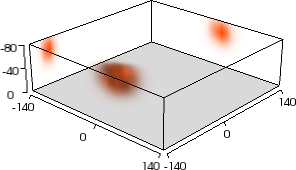
\includegraphics[width=4.5cm]{plots/vis_gaussian}\label{fig:SS-G}}%
    \subfigure[Single source 
    dispersion]{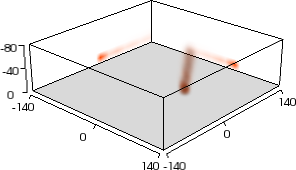
\includegraphics[width=4.5cm]{plots/vis_dispersion}\label{fig:SS-D}}%
    \subfigure[Multiple source 
    dispersion]{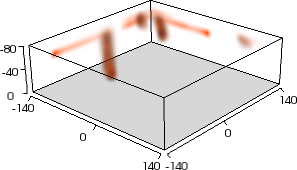
\includegraphics[width=4.5cm]{plots/vis_multi_dispersion}\label{fig:MS-D}}
    \caption[Visualizations of plume dispersions]{Visualization of different 
        plume dispersions. The rear boundaries of the volume show 
        two-dimensional projections of concentration maxima in the respective 
        directions. Axes scale is in meters.}
\end{figure}

A Gaussian dispersion (D) as shown in Figure~\ref{fig:SS-D} is obtained when 
considering a constant wind parallel to the ground with velocity $u$ measured 
\SI{6}{\meter} above the ground. The plume will be dispersed and form 
a cone-like distribution along the wind direction.  Making a few more 
assumptions (constant $Q$, steady-state, isotropic diffusion, no ground 
penetration, and neglegible variation in topography) the analytic expression
\begin{multline}\label{eqn:plumedisp}
    c(\vc x') = \frac{Q}{2\uppi ua\del{x'_1 - s'_1}^b} 
    \exp\!\del{-\frac{\del{x'_2 - s'_2}^2}{2a\del{x'_1 - s'_1}^b}} \\ 
    \sbr{\exp\!\del{-\frac{\del{x'_3 - s'_3}^2}{2a\del{x'_1 - s'_1}^b}} 
        + \exp\!\del{-\frac{\del{x'_3 + s'_3}^2}{2a\del{x'_1 - s'_1}^b}}}
\end{multline}
can be derived for the concentration \parencite{Stockie:2011fd}. Note that the 
coordinates $\vc x'$ and $\vc s'$ are expressed in the wind frame of reference.  
In the dispersion scenarios the wind speed is set to $u 
= \SI{3}{\meter\per\second}$ and the diffusion parameters to $a 
= \SI{0.33}{\meter\tothe{2 - \mathit{b}}}$ and $b = 0.86$.  The emission rate 
$Q$ is randomly chosen from a uniform distribution over the interval 
\SIrange{0.1}{2.5}{\gram\per\second}.

Sensor noise (SN) of the plume sensor is assumed to be additive and distributed 
according to $\mathcal{N}(0, \sigma\ped{sn}^2)$. In the noise free (NF) 
scenarios no noise was added to the measurements. The standard deviation 
$\sigma\ped{sn}$ was set to $\SI{e-5}{\gram\per\meter\cubed}$ in the scenarios 
including noise.  The QRSim default scenarios set it to 
$\SI{e-2}{\gram\per\meter\cubed}$, but given the low default plume concentration 
this would require roughly an averaging of 385 samples from one single location 
to reduce the magnitude of the noise below the magnitude of the concentration 
values (see Appendix~\ref{sec:decnoise}).  Hence, the default scenario is not 
solvable in a feasible amount of simulation time.

The overall concentration $c(\vc x)$ for $n$ sources like in 
Figure~\ref{fig:MS-D} is obtained by summing the individual contributions 
$c_i(\vc x)$ of each source:
\begin{equation}
    c(\vc x) = \sum_{i = 1}^n c_i(\vc x)
\end{equation}
In the scenarios with multiple sources (MS) $n$ is chosen uniformly out of the 
range from \numrange{1}{5}. With a single source (SS) $n = 1$ is fixed. In both 
cases the source locations will be randomly chosen from a uniform distribution 
over the simulated volume.

The starting locations of the UAVs are also chosen randomly and uniformly in the 
simulated area, but the height is initially set to $x_3 = \SI{-10}{\meter}$.  
Either a single UAV (SV) or three UAVs (MV) were used.

This gives a number of possible scenarios from which I focussed on the following 
in this work:
\begin{itemize}
    \item In Chapter~\ref{sec:cmputility} I discuss the noise free, single 
        vehicle scenarios G-NF-SS-SV, D-NF-SS-SV, and D-NF-MS-SV\@. The first is 
        equivalent to the scenario 3A in \textcite{denardi2013rn}.
    \item In Chapter~\ref{sec:noisy} I consider the dispersion scenarios with 
        noise D-SN-SS-SV and D-SN-MS-SV\@. Except for the amount of noise these 
        correspond to scenarios 3B and 3C in \textcite{denardi2013rn}.
    \item Finally, I will take a look at the usage of multiple vehicles with the 
        scenario D-SN-MS-MV corresponding to scenario 3D in 
        \textcite{denardi2013rn}.
\end{itemize}
